% Options for packages loaded elsewhere
\PassOptionsToPackage{unicode}{hyperref}
\PassOptionsToPackage{hyphens}{url}
\PassOptionsToPackage{dvipsnames,svgnames,x11names}{xcolor}
%
\documentclass[
  12pt,
]{article}
\usepackage{amsmath,amssymb}
\usepackage{lmodern}
\usepackage{iftex}
\ifPDFTeX
  \usepackage[T1]{fontenc}
  \usepackage[utf8]{inputenc}
  \usepackage{textcomp} % provide euro and other symbols
\else % if luatex or xetex
  \usepackage{unicode-math}
  \defaultfontfeatures{Scale=MatchLowercase}
  \defaultfontfeatures[\rmfamily]{Ligatures=TeX,Scale=1}
\fi
% Use upquote if available, for straight quotes in verbatim environments
\IfFileExists{upquote.sty}{\usepackage{upquote}}{}
\IfFileExists{microtype.sty}{% use microtype if available
  \usepackage[]{microtype}
  \UseMicrotypeSet[protrusion]{basicmath} % disable protrusion for tt fonts
}{}
\usepackage{xcolor}
\usepackage[margin=1in]{geometry}
\usepackage{graphicx}
\makeatletter
\def\maxwidth{\ifdim\Gin@nat@width>\linewidth\linewidth\else\Gin@nat@width\fi}
\def\maxheight{\ifdim\Gin@nat@height>\textheight\textheight\else\Gin@nat@height\fi}
\makeatother
% Scale images if necessary, so that they will not overflow the page
% margins by default, and it is still possible to overwrite the defaults
% using explicit options in \includegraphics[width, height, ...]{}
\setkeys{Gin}{width=\maxwidth,height=\maxheight,keepaspectratio}
% Set default figure placement to htbp
\makeatletter
\def\fps@figure{htbp}
\makeatother
\setlength{\emergencystretch}{3em} % prevent overfull lines
\providecommand{\tightlist}{%
  \setlength{\itemsep}{0pt}\setlength{\parskip}{0pt}}
\setcounter{secnumdepth}{5}
\newlength{\cslhangindent}
\setlength{\cslhangindent}{1.5em}
\newlength{\csllabelwidth}
\setlength{\csllabelwidth}{3em}
\newlength{\cslentryspacingunit} % times entry-spacing
\setlength{\cslentryspacingunit}{\parskip}
\newenvironment{CSLReferences}[2] % #1 hanging-ident, #2 entry spacing
 {% don't indent paragraphs
  \setlength{\parindent}{0pt}
  % turn on hanging indent if param 1 is 1
  \ifodd #1
  \let\oldpar\par
  \def\par{\hangindent=\cslhangindent\oldpar}
  \fi
  % set entry spacing
  \setlength{\parskip}{#2\cslentryspacingunit}
 }%
 {}
\usepackage{calc}
\newcommand{\CSLBlock}[1]{#1\hfill\break}
\newcommand{\CSLLeftMargin}[1]{\parbox[t]{\csllabelwidth}{#1}}
\newcommand{\CSLRightInline}[1]{\parbox[t]{\linewidth - \csllabelwidth}{#1}\break}
\newcommand{\CSLIndent}[1]{\hspace{\cslhangindent}#1}
\usepackage{setspace} \setstretch{1.15} \usepackage{float} \floatplacement{figure}{t}
\usepackage{booktabs}
\usepackage{longtable}
\usepackage{array}
\usepackage{multirow}
\usepackage{wrapfig}
\usepackage{float}
\usepackage{colortbl}
\usepackage{pdflscape}
\usepackage{tabu}
\usepackage{threeparttable}
\usepackage{threeparttablex}
\usepackage[normalem]{ulem}
\usepackage{makecell}
\usepackage{xcolor}
\ifLuaTeX
  \usepackage{selnolig}  % disable illegal ligatures
\fi
\IfFileExists{bookmark.sty}{\usepackage{bookmark}}{\usepackage{hyperref}}
\IfFileExists{xurl.sty}{\usepackage{xurl}}{} % add URL line breaks if available
\urlstyle{same} % disable monospaced font for URLs
\hypersetup{
  pdftitle={test},
  pdfauthor={Angelos Vasilopoulos; Gregory J. Matthews},
  colorlinks=true,
  linkcolor={cyan},
  filecolor={Maroon},
  citecolor={Blue},
  urlcolor={cyan},
  pdfcreator={LaTeX via pandoc}}

\title{test}
\author{Angelos Vasilopoulos \and Gregory J. Matthews}
\date{}

\begin{document}
\maketitle
\begin{abstract}
Abstract \vspace{2mm}\\
\emph{Keywords}: Cross validation
\end{abstract}

\newpage

\hypertarget{sec:intro}{%
\section{Introduction}\label{sec:intro}}

\(k\)-fold cross-validation is a popular method of error estimation for
model selection in computational research.

n observations are divided into \(k\) groups. In a first iteration,
\(i = k - 1\) groups are used as a training set. The remaining group is
used as a test set to estimate prediction error. This process is
repeated \(i\) times, with a different test set in each iteration. The
average of \(k\) prediction errors (\(PE\))
\[\hat{\theta} = CV_{(k)} = \frac{1}{k}\sum_{i=1}^{k}PE_i\]

is meant to estimate the true model error \(\theta\), i.e., the error of
the model tested on the population.

Despite the popularity of cross-validation, there is limited focus in
the literature on the question of what fold number \(k\) is appropriate
for cross-validation with a given data set. One popular idea is that
selection of \(k\) comes with a bias-variance trade-off, specifically,
that as \(k\) increases, the bias of k-fold error estimation
\[Bias(\hat{\theta}) = E(\hat{\theta}) - \theta\] and variance of
\(k\)-fold error estimation
\[Var(\hat{\theta}) = E(\hat{\theta}^2) - E(\hat{\theta})^2\] as in
\[Err(\hat{\theta}) = Bias^2(\hat{\theta}) + Var(\hat{\theta})\]
decrease and increase, respectively. This idea appears in early
literature (Efron (\protect\hyperlink{ref-Efron1983}{1983}); Kohavi
(\protect\hyperlink{ref-Kohavi2001}{2001})).

Subsequent, albeit limited, literature argues differently. In the case
of leave-one-out cross-validation, i.e., with \(k\) = 1, previous
literature suggests that asymptotically both bias and variance of error
estimation decrease as \(k\) increases (Burman
(\protect\hyperlink{ref-Burman1989}{1989})) and that bias and variance
of error estimation are uniformly low (Breiman and Spector
(\protect\hyperlink{ref-Breiman1992}{1992})).

More recently have been proposed ways to quantify the variance reduction
achieved by cross-validation when the true prediction error is not
known, e.g., as mean-square stability (Kale, Kumar, and Vassilvitskii
(\protect\hyperlink{ref-Kale2011}{2011})), which measures performance
estimate variance across folds, or as loss stability (Kumar et al.
(\protect\hyperlink{ref-Kumar2013}{2013})), the proportion of times that
a model outperforms competing models in all folds. However, it has also
been demonstrated that, due to overlap between training and test sets in
cross-validation, there is no universal (i.e., valid under all
distributions) unbiased estimator of the variance of \(k\)-fold cross
validation (Bengio and Grandvalet
(\protect\hyperlink{ref-Bengio2004}{2004})).

In addition to theoretical analysis of variance reduction by cross
validation, there are some simulation results showing this phenomenon
(Zhang and Yang (\protect\hyperlink{ref-Zhang2015}{2015})). However,
simulations currently in the literature provide limited insight into the
dependence of optimal fold number \(k\) on sample size \(n\). Here we
present a simulation of linear regression and least absolute shrinkage
and regression operator (LASSO) regression to observe the relationship
of cross-validation fold number \(k\) and model prediction error
estimation accuracy for various sample sizes \(n\).

\hypertarget{simulation}{%
\section{Simulation}\label{simulation}}

Consider a population of size \(N = 500,000\) with five of 100 features
\(X \sim N(0, 1)\) a linear combination
\[Y = \beta_0 + \beta_1X_1 + \beta_2X_2 + \beta_3X_3 + \beta_4X_4 + \beta_5X_5 + \epsilon\]
where \(\beta_1...\beta_5 = 1\) and \(\epsilon \sim N(0, 10)\). Then the
true model of the population is
\[E(Y) = \beta_0 + \beta_1X_1 + \beta_2X_2 + \beta_3X_3 + \beta_4X_4 + \beta_5X_5\]
and the mean squared error (\(MSE\)) of the true model is
\[MSE[E(Y)] = \theta = \frac{\sum_{i=1}^{N}[Y - E(Y)]^2}{N}.\]

From the population we take a sample of size \(n\). We estimate \(Y\) as
\(\hat{Y}\) by regression on a subset of \(X\) and estimate
\(MSE(\hat{Y})\) as
\[\hat{\theta} = \frac{\sum_{i=1}^{N}(Y - \hat{Y})^2}{N}\] by \(k\)-fold
cross-validation. We repeat this procedure in 1000 simulations for the
same subsets of \(X\), including the five-variable subset of the true
model, and values of \(k\). We then calculate simulation-wise
\(MSE(\hat{\theta})\) for each value of \(k\).

We perform an additional 1000 simulations predicting \(Y\) as
\(\hat{Y}\) by LASSO regression instead of linear regression. To avoid
data leakage, we introduce an inner 5-fold cross-validation loop for the
selection of regularization parameter \(\lambda\) as in the minimization
of
\[\sum_{i=1}^{n}(Y_i - \sum_{j}X_{ij}\beta_j)^2 + \lambda\sum_{j=1}^{p}|\beta_j|.\]

We perform the same 1000 simulations with \(n\) = \{100, 500, 1000\} and
consider as the optimal value of \(k\) the value \(k_{optimal}\)
resulting in the lowest \(MSE(\hat{\theta})\) for the true model the
greatest number of times.

This is because in practice the model with the lowest prediction error
is more likely to be selected. We refer to this as lowest-error model
selection. As our simulation results show, however, it is possible for
\(k\)-fold cross validation to result in calculations of
\(MSE(\hat{\theta})\) that suggest that a competing model has a lower
prediction error than the true model. This false model may have the
lowest prediction error in \(k\)-fold cross validation but its
generalization error will be lower in the long-run (i.e., when tested on
a large part of the population) than the generalization error of the
true model, as \(E(Y)\) is a linear combination of the true model only.
Thus, it is preferable for the value of \(k\) selected to result in the
true model having the lowest estimated prediction error.

\hypertarget{results}{%
\section{Results}\label{results}}

We find that for all \(n\) as fold number \(k\) increases, both bias and
variance of error estimation decrease initially before leveling off
(Figures 1 - 3).

\begin{center}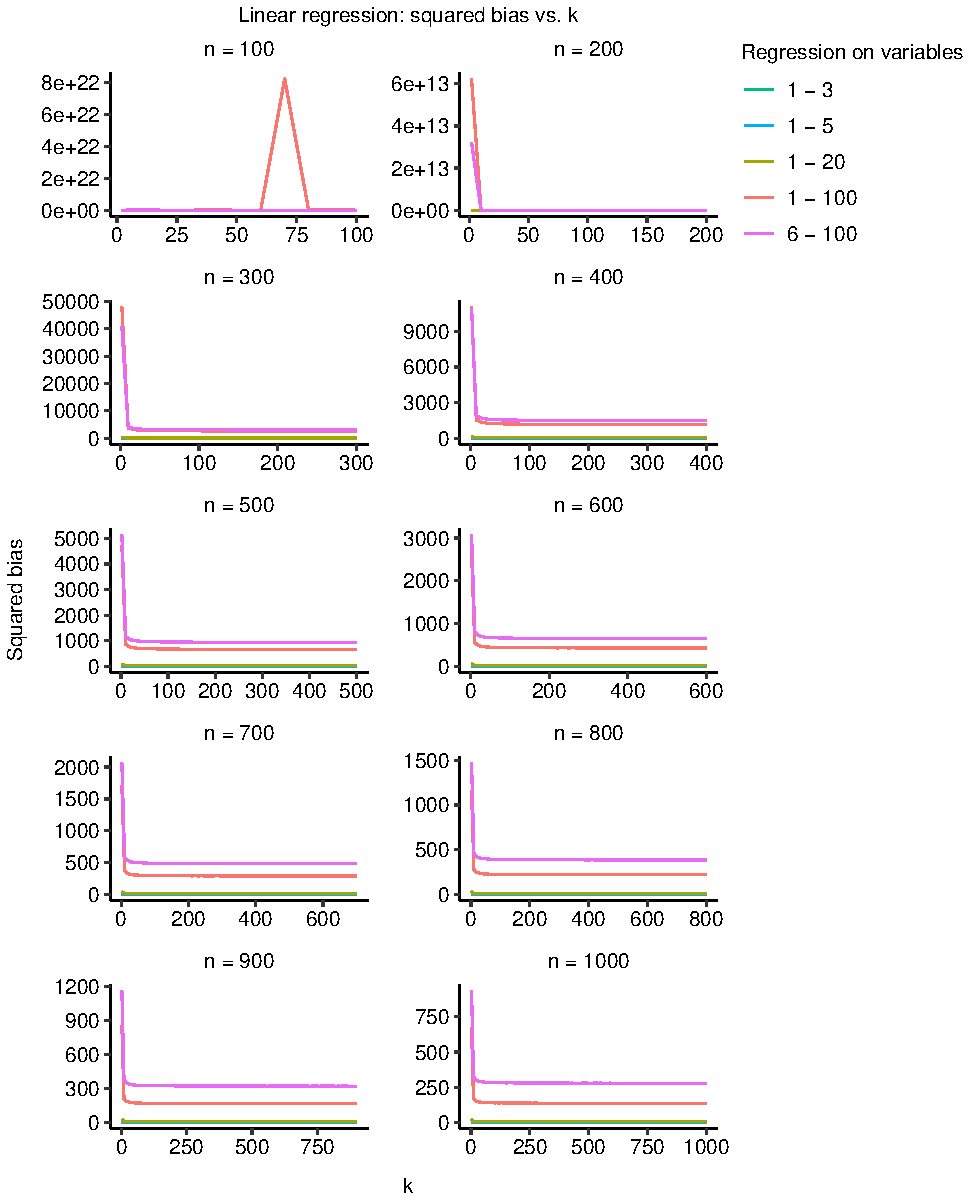
\includegraphics{manuscript_files/figure-latex/unnamed-chunk-1-1} \end{center}

\begin{center}\includegraphics{manuscript_files/figure-latex/unnamed-chunk-1-2} \end{center}

\begin{center}\includegraphics{manuscript_files/figure-latex/unnamed-chunk-1-3} \end{center}

We also find that for larger \(n\), e.g., \(n = 1000\), lowest-error
model selection becomes less reliable as \(k\) increases past a certain
value, i.e., as \(k\) increases past a certain value the true model has
the lowest MSE less frequently. With increasing \(n\) we also observe
variability in the improvement of lowest-error model selection
reliability (Figure 4; Table 1).

\begin{center}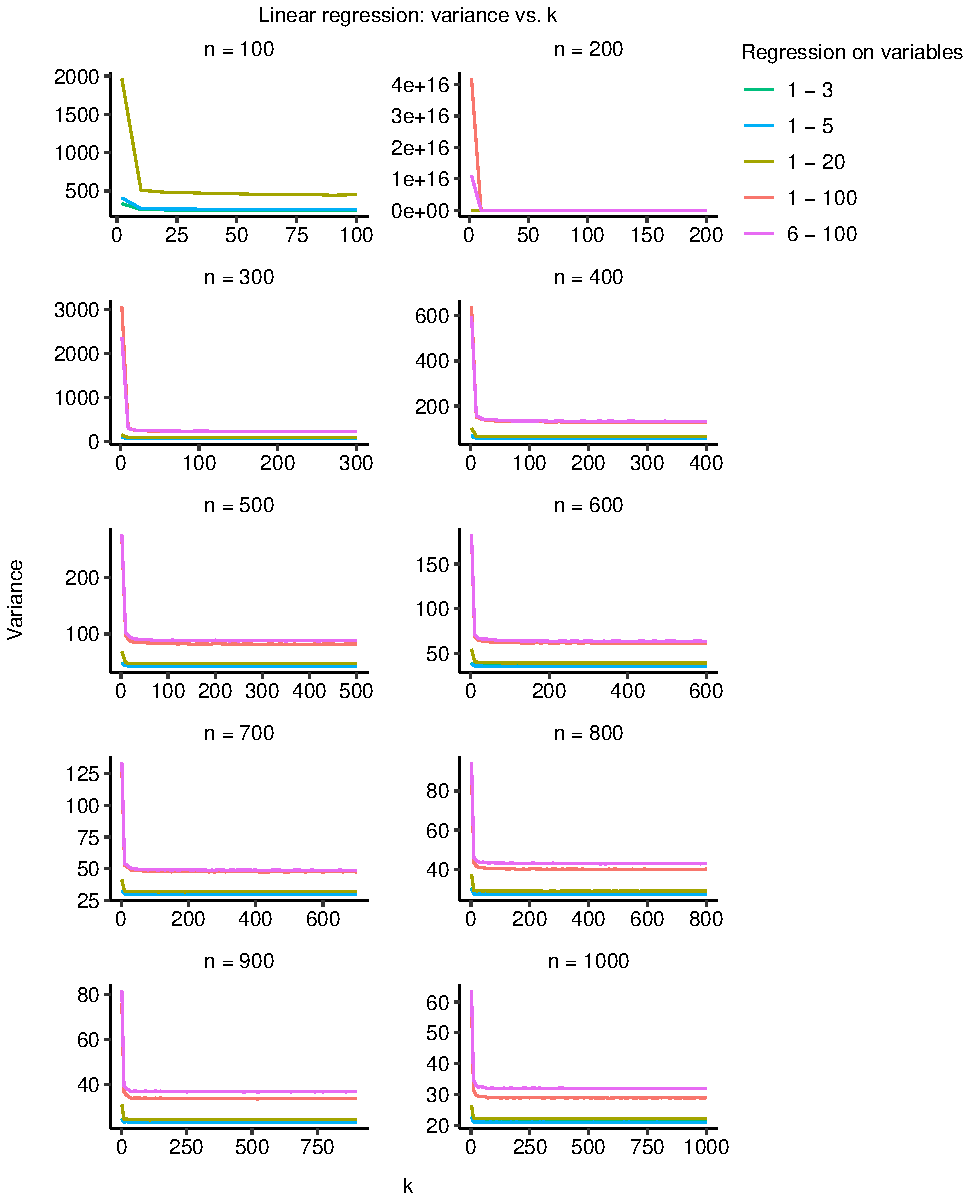
\includegraphics{manuscript_files/figure-latex/unnamed-chunk-2-1} \end{center}
\begin{table}[!h]
\centering
\begin{tabular}{r|r|r|r|r}
\hline
n & Minimum & Maximum & Range & Variance\\
\hline
100 & 240 & 306 & 66 & 140.0310\\
\hline
250 & 386 & 500 & 114 & 427.1585\\
\hline
500 & 619 & 813 & 194 & 676.5341\\
\hline
1000 & 861 & 931 & 70 & 711.2000\\
\hline
\end{tabular}
\end{table}

\hypertarget{conclusion}{%
\section{Conclusion}\label{conclusion}}

Early literature suggests that increasing cross-validation fold number
is related to decreasing bias and increasing variance of error
estimation. However, more recent work suggests that this is not the
case. Instead, increasing \(k\) results in bias and variance reduction.
This phenomenon is observable in our simulation results, although it is
also clear from the results that the reductions are not limitless,
meaning that there is a point of diminishing returns in increasing \(k\)
and computational power allocation, as error estimation does not improve
after a certain value of \(k\).

Our results also indicate a relationship between optimal fold number
\(k\) and sample size \(n\), although more data is necessary to
elucidate a trend. This is interesting as a future direction, as
modeling the relationship between \(n\) and \(k_{optimal}\) would have
practical utility, potentially improving the selection of \(k\) from a
largely arbitrary decision between 5 and 10. Future research may also
focus on error estimation of other models, including models capturing
non-linear relationships or involving tuning of multiple
hyper-parameters, e.g., random forest or gradient boosting.

\hypertarget{acknowledgements}{%
\section*{Acknowledgements}\label{acknowledgements}}
\addcontentsline{toc}{section}{Acknowledgements}

Dr.~Gregory Matthews's Fall 2022 Predictive Analytics class.

\hypertarget{supplementary-material}{%
\section*{Supplementary Material}\label{supplementary-material}}
\addcontentsline{toc}{section}{Supplementary Material}

All code for reproducing the analyses in this paper is publicly
available at \url{https://github.com/gjm112/optimal_k}.

\hypertarget{references}{%
\section*{References}\label{references}}
\addcontentsline{toc}{section}{References}

\hypertarget{refs}{}
\begin{CSLReferences}{1}{0}
\leavevmode\vadjust pre{\hypertarget{ref-Bengio2004}{}}%
Bengio, Yoshua, and Yves Grandvalet. 2004. {``No Unbiased Estimator of
the Variance of k-Fold Cross-Validation,''} June.

\leavevmode\vadjust pre{\hypertarget{ref-Breiman1992}{}}%
Breiman, Leo, and Philip Spector. 1992. {``Submodel Selection and
Evaluation in Regression. The x-Random Case.''} \emph{International
Statistical Review / Revue Internationale de Statistique} 60 (3): 291.
\url{https://doi.org/10.2307/1403680}.

\leavevmode\vadjust pre{\hypertarget{ref-Burman1989}{}}%
Burman, Prabir. 1989. {``A Comparative Study of Ordinary
Cross-Validation, v-Fold Cross-Validation and the Repeated
Learning-Testing Methods.''} \emph{Biometrika} 76 (September): 503--14.
\url{https://doi.org/10.1093/biomet/76.3.503}.

\leavevmode\vadjust pre{\hypertarget{ref-Efron1983}{}}%
Efron, Bradley. 1983. {``Estimating the Error Rate of a Prediction Rule:
Improvement on Cross-Validation.''} \emph{Journal of the American
Statistical Association} 78 (382): 316--31.
\url{https://doi.org/10.1080/01621459.1983.10477973}.

\leavevmode\vadjust pre{\hypertarget{ref-Kale2011}{}}%
Kale, Satyen, Ravi Kumar, and Sergei Vassilvitskii. 2011.
{``Cross-Validation and Mean-Square Stability.''} In, 487--95.

\leavevmode\vadjust pre{\hypertarget{ref-Kohavi2001}{}}%
Kohavi, Ron. 2001. {``A Study of Cross-Validation and Bootstrap for
Accuracy Estimation and Model Selection''} 14 (March).

\leavevmode\vadjust pre{\hypertarget{ref-Kumar2013}{}}%
Kumar, Ravi, Daniel Lokshtanov, Sergei Vassilvitskii, and Andrea
Vattani. 2013. {``Near-Optimal Bounds for Cross-Validation via Loss
Stability.''} In \emph{Proceedings of the 30th International Conference
on Machine Learning}, edited by Sanjoy Dasgupta and David McAllester,
28:27--35. Proceedings of Machine Learning Research 1. Atlanta, Georgia,
USA: PMLR. \url{https://proceedings.mlr.press/v28/kumar13a.html}.

\leavevmode\vadjust pre{\hypertarget{ref-Zhang2015}{}}%
Zhang, Yongli, and Yuhong Yang. 2015. {``Cross-Validation for Selecting
a Model Selection Procedure.''} \emph{Journal of Econometrics} 187 (1):
95--112. \url{https://doi.org/10.1016/j.jeconom.2015.02.006}.

\end{CSLReferences}

\end{document}
